\documentclass[11pt]{article}
\usepackage[utf8]{inputenc}
\usepackage{fullpage,amsmath,amsthm,enumerate}
\usepackage[citecolor=blue,linkcolor=blue,colorlinks=true]{hyperref}
\usepackage{tikz}
\usepackage{graphicx}
\usepackage{xcolor}  % To color a text in 
\usepackage{multicol} % For multiple columns
\usepackage{caption}
\usepackage{subcaption}
\counterwithin{table}{subsection}
\counterwithin{figure}{subsection}

% Theorems
\newtheorem{theorem}{Theorem}
\newtheorem{lemma}{Lemma}

% Commands
\newcommand{\calF}{$\mathcal{F}$}
\newcommand{\set}[1]{\{ #1 \}}
\newcommand{\zon}{$\{0,1\}^n$}
\newcommand{\zo}{$\{0,1\}$}

\title{Classification (Using Discriminative models)\\
Report}
\author{Reetwik Das}

\begin{document}
\maketitle
\newpage
\tableofcontents
\listoftables
\listoffigures

\newpage 

\section{Dataset 1a}
\subsection{Perceptron for every pair of class}
Hyperparameter $\eta = \{0.1,0.5,1\}$\\

Since the classes are linearly well separated we got the same accuracies for each value of $\eta$.
\begin{table}[h!]
\label{tab:tab1.1.1}
\begin{center}
\begin{tabular}{|l|c|c|c|}
\hline
\textbf{classes} & \textbf{Training Dataset} & \textbf{Validation Dataset} &\textbf{Test Dataset}\\
\hline
0 vs 1 & 100 & 100 & 100\\
\hline
0 vs 2 & 100 & 100 & 100\\
\hline
0 vs 3 & 100 & 100 & 100\\
\hline
1 vs 2 & 100 & 100 & 100\\
\hline
1 vs 3 & 100 & 100 & 100\\
\hline
2 vs 3 & 100 & 100 & 100\\
\hline
\end{tabular}
\caption{Classification accuracy using perceptron on Dataset 1a}
\end{center}
\end{table}

As we can see from the table above the model with the best performance on the test data is with  $\eta =1$ with an accuracy of 100\% for each pair of class .
\begin{figure}[h]
\centering
	\begin{subfigure}[b]{0.45\textwidth}
	\centering
	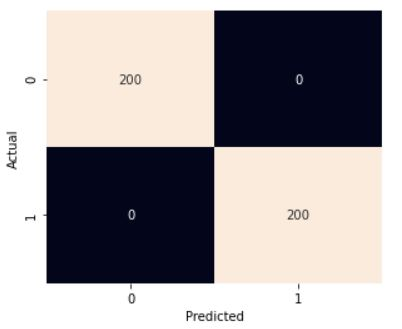
\includegraphics[scale=0.45]{dataset1a_perceptron_01_cm_train.jpg}
	\caption{Training data}
	\label{fig:fig1.1.1.1}
	\end{subfigure}
	\begin{subfigure}[b]{0.45\textwidth}
	\centering
	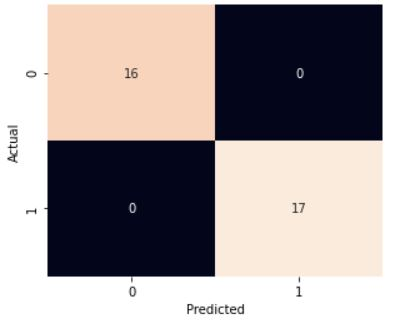
\includegraphics[scale=0.45]{dataset1a_perceptron_01_cm_test.jpg}
	\caption{Test data}
	\label{fig:fig1.1.1.2}
	\end{subfigure}
\caption{Confusion matrix for the classification between class 0 vs class 1 of dataset 1a using Perceptron}
\label{fig:fig1.1.1}
\end{figure}

\begin{figure}[h]
\centering
	\begin{subfigure}[b]{0.45\textwidth}
	\centering
	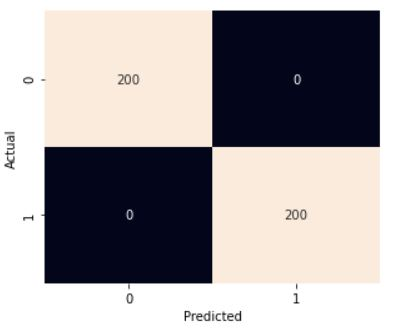
\includegraphics[scale=0.45]{dataset1a_perceptron_02_cm_train.jpg}
	\caption{Training data}
	\label{fig:fig1.1.2.1}
	\end{subfigure}
	\begin{subfigure}[b]{0.45\textwidth}
	\centering
	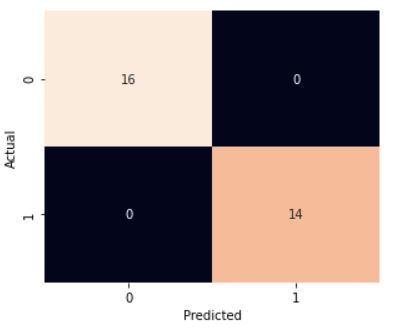
\includegraphics[scale=0.45]{dataset1a_perceptron_02_cm_test.jpg}
	\caption{Test data}
	\label{fig:fig1.1.2.2}
	\end{subfigure}
\caption{Confusion matrix for the classification between class 0 vs class 2 of dataset 1a using Perceptron}
\label{fig:fig1.1.2}
\end{figure}

\begin{figure}
\centering
	\begin{subfigure}[b]{0.45\textwidth}
	\centering
	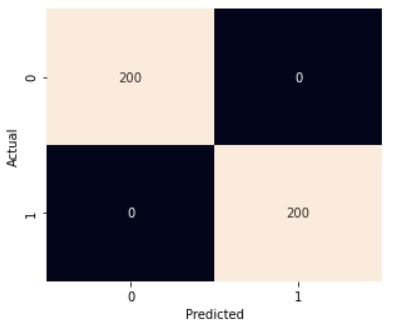
\includegraphics[scale=0.4]{dataset1a_perceptron_03_cm_train.jpg}
	\caption{Training data}
	\label{fig:fig1.1.3.1}
	\end{subfigure}
	\begin{subfigure}[b]{0.45\textwidth}
	\centering
	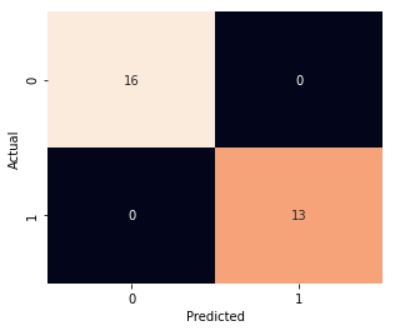
\includegraphics[scale=0.4]{dataset1a_perceptron_03_cm_test.jpg}
	\caption{Test data}
	\label{fig:fig1.1.3.2}
	\end{subfigure}
\caption{Confusion matrix for the classification between class 0 vs class 3 of dataset 1a using Perceptron}
\label{fig:fig1.1.3}
\end{figure}

\begin{figure}
\centering
	\begin{subfigure}[b]{0.45\textwidth}
	\centering
	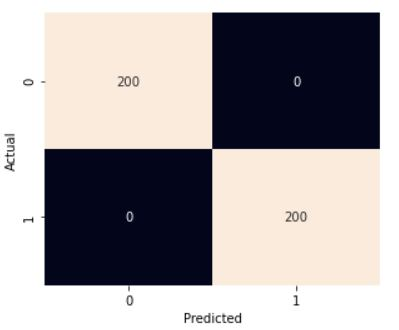
\includegraphics[scale=0.4]{dataset1a_perceptron_12_cm_train.jpg}
	\caption{Training data}
	\label{fig:fig1.1.4.1}
	\end{subfigure}
	\begin{subfigure}[b]{0.45\textwidth}
	\centering
	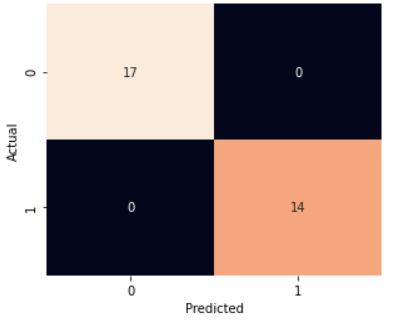
\includegraphics[scale=0.4]{dataset1a_perceptron_12_cm_test.jpg}
	\caption{Test data}
	\label{fig:fig1.1.4.2}
	\end{subfigure}
\caption{Confusion matrix for the classification between class 1 vs class 2 of dataset 1a using Perceptron}
\label{fig:fig1.1.4}
\end{figure}

\begin{figure}
\centering
	\begin{subfigure}[b]{0.45\textwidth}
	\centering
	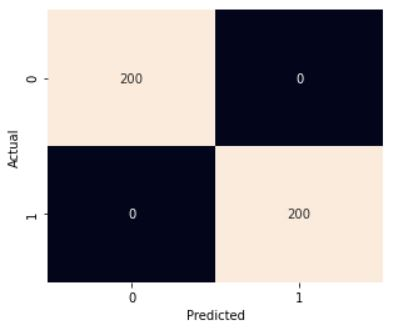
\includegraphics[scale=0.4]{dataset1a_perceptron_13_cm_train.jpg}
	\caption{Training data}
	\label{fig:fig1.1.5.1}
	\end{subfigure}
	\begin{subfigure}[b]{0.45\textwidth}
	\centering
	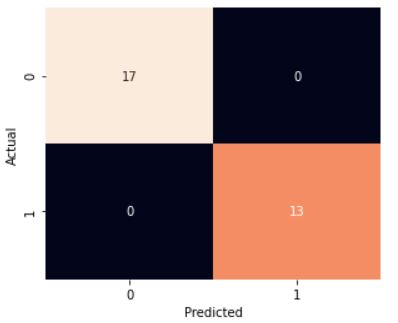
\includegraphics[scale=0.4]{dataset1a_perceptron_13_cm_test.jpg}
	\caption{Test data}
	\label{fig:fig1.1.5.2}
	\end{subfigure}
\caption{Confusion matrix for the classification between class 1 vs class 3 of dataset 1a using Perceptron}
\label{fig:fig1.1.5}
\end{figure}

\begin{figure}
\centering
	\begin{subfigure}[b]{0.45\textwidth}
	\centering
	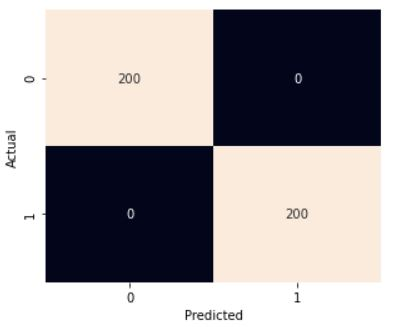
\includegraphics[scale=0.4]{dataset1a_perceptron_23_cm_train.jpg}
	\caption{Training data}
	\label{fig:fig1.1.6.1}
	\end{subfigure}
	\begin{subfigure}[b]{0.45\textwidth}
	\centering
	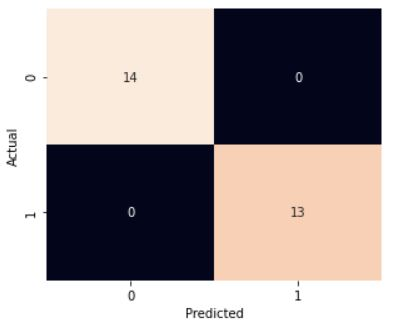
\includegraphics[scale=0.4]{dataset1a_perceptron_23_cm_test.jpg}
	\caption{Test data}
	\label{fig:fig1.1.6.2}
	\end{subfigure}
\caption{Confusion matrix for the classification between class 2 vs class 3 of dataset 1a using Perceptron}
\label{fig:fig1.1.6}
\end{figure}

\newpage
\begin{figure}[h]
\centering
	\begin{subfigure}[b]{0.45\textwidth}
	\centering
	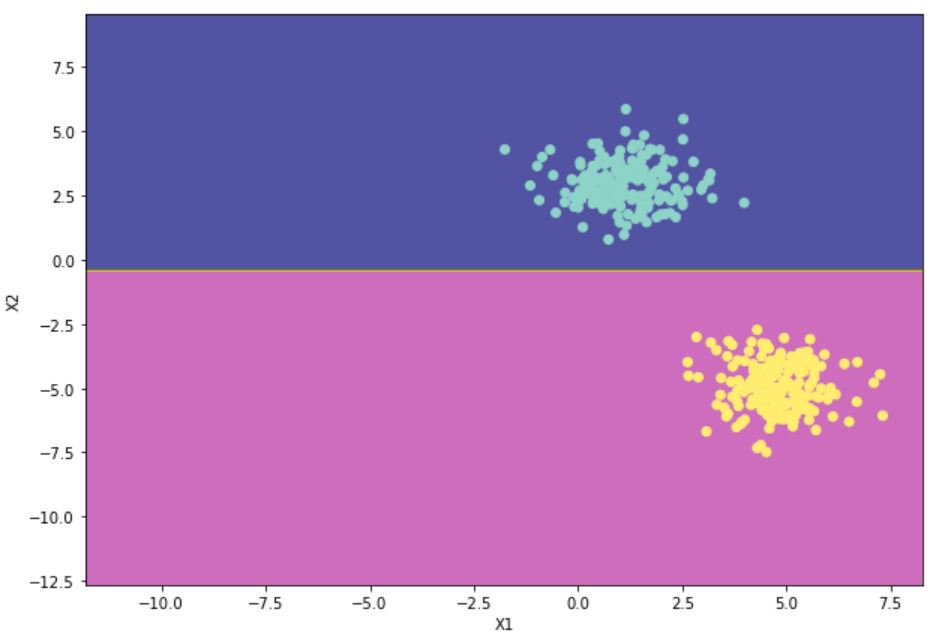
\includegraphics[scale=0.3]{dataset1a_perceptron_01_ds.jpg}
	\caption{class 0 vs class 1}
	\label{fig:fig1.1.7.1}
	\end{subfigure}
	\begin{subfigure}[b]{0.45\textwidth}
	\centering
	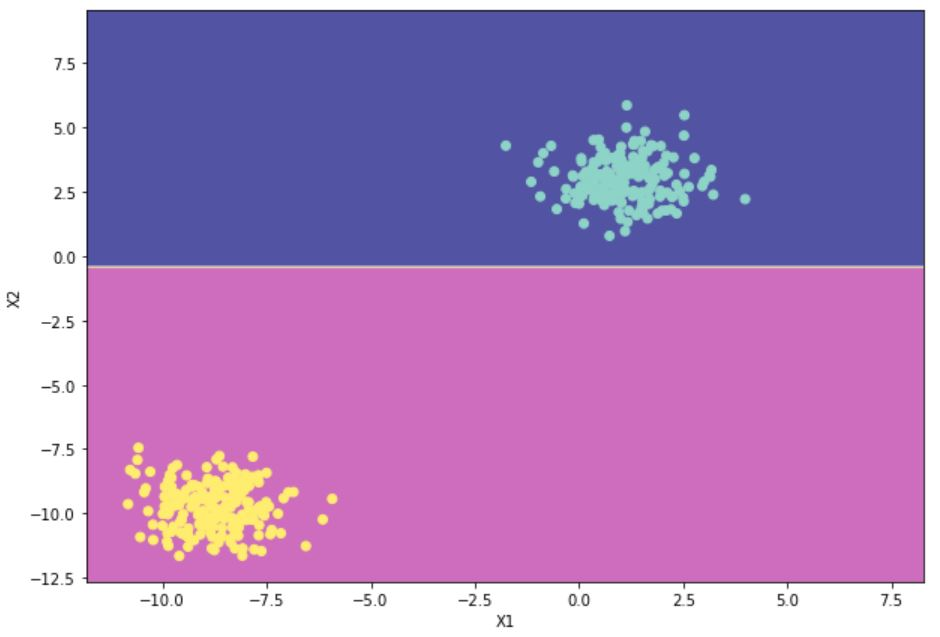
\includegraphics[scale=0.3]{dataset1a_perceptron_02_ds.jpg}
	\caption{class 0 vs class 2}
	\label{fig:fig1.1.7.2}
	\end{subfigure}
	\begin{subfigure}[b]{0.45\textwidth}
	\centering
	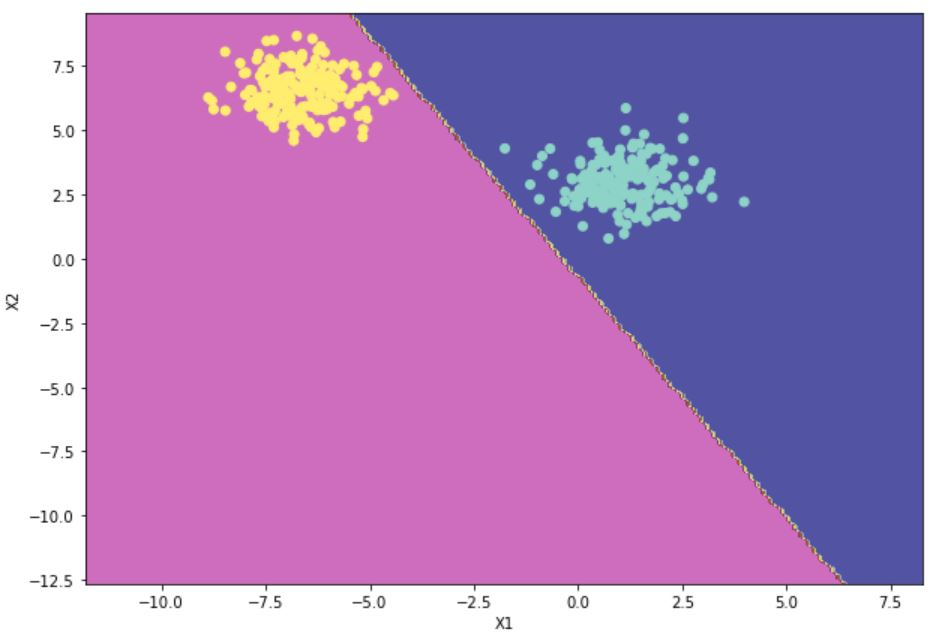
\includegraphics[scale=0.3]{dataset1a_perceptron_03_ds.jpg}
	\caption{class 0 vs class 3}
	\label{fig:fig1.1.7.3}
	\end{subfigure}
	\begin{subfigure}[b]{0.45\textwidth}
	\centering
	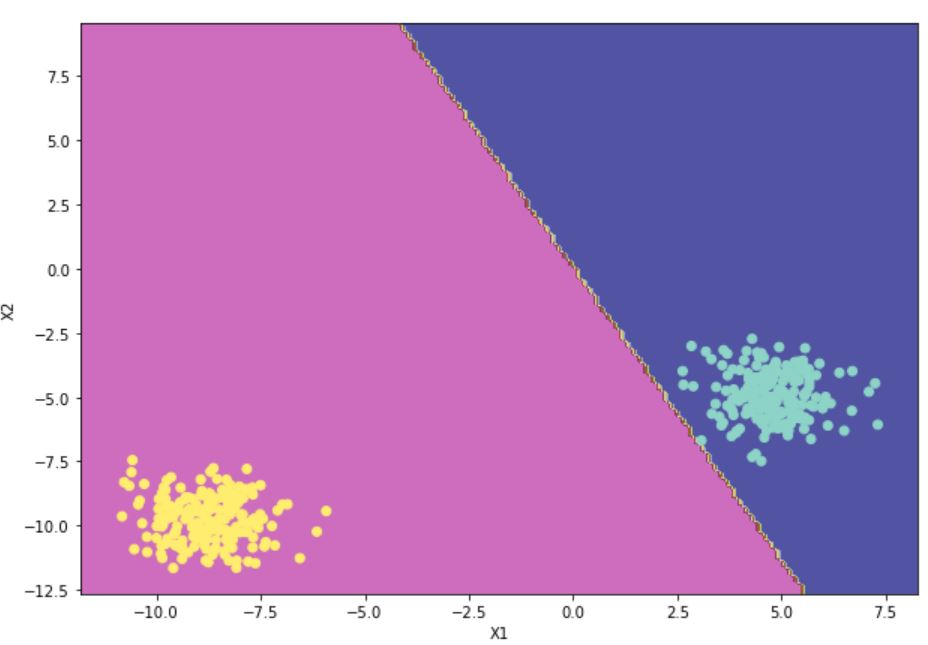
\includegraphics[scale=0.3]{dataset1a_perceptron_12_ds.jpg}
	\caption{class 1 vs class 2}
	\label{fig:fig1.1.7.4}
	\end{subfigure}
	\begin{subfigure}[b]{0.45\textwidth}
	\centering
	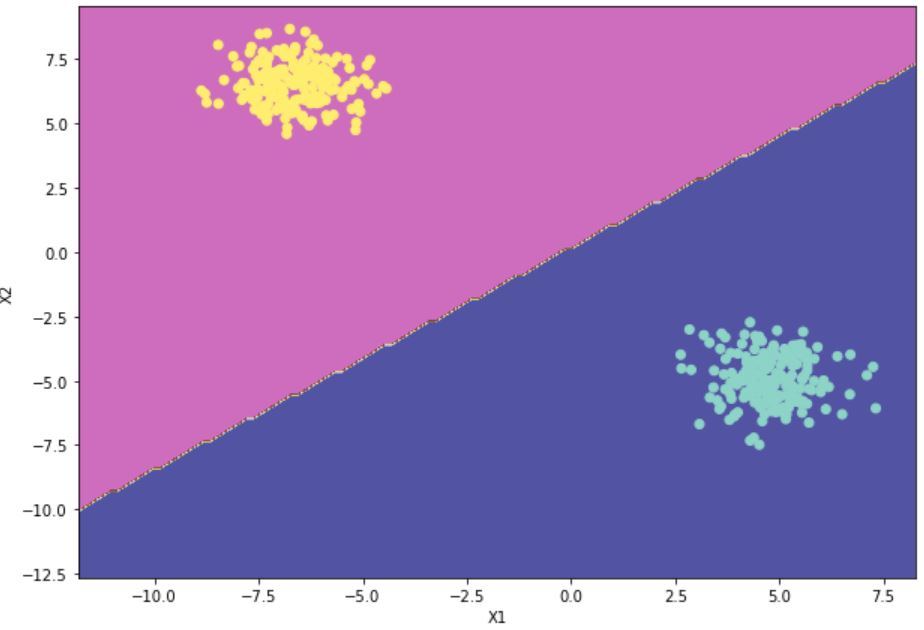
\includegraphics[scale=0.3]{dataset1a_perceptron_13_ds.jpg}
	\caption{class 1 vs class 3}
	\label{fig:fig1.1.7.5}
	\end{subfigure}
	\begin{subfigure}[b]{0.45\textwidth}
	\centering
	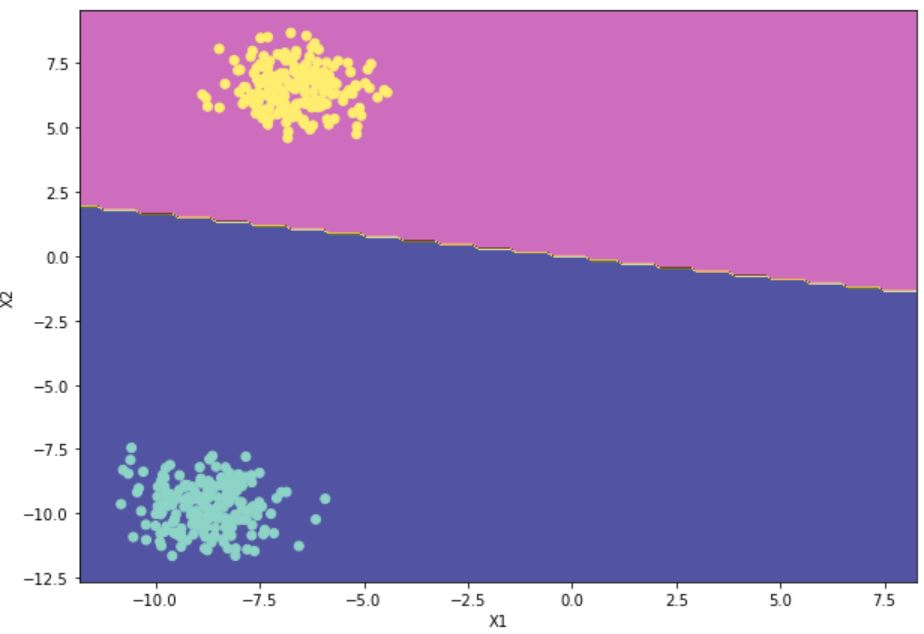
\includegraphics[scale=0.3]{dataset1a_perceptron_23_ds.jpg}
	\caption{class 2 vs class 3}
	\label{fig:fig1.1.7.6}
	\end{subfigure}
\caption{Decision region plots between each pair of classes of dataset 1a using Perceptron}
\label{fig:fig1.1.7}
\end{figure}

We observe that since the classes are well separated we are clearly able to classify them using perceptron with very high accuracy.

\newpage

\subsection{MLFFNN with single hidden layer for all classes}
Hyperparameter no. of nodes in the hidden layer $= \{3,4,5\}$\\

Since the classes are linearly well separated we got the same accuracies for each value of number of nodes. We used a learning rate $\eta = 0.001$, $\alpha = 1$. 
\begin{table}[h!]
\label{tab:tab1.2.1}
\begin{center}
\begin{tabular}{|l|c|c|c|}
\hline
\textbf{\# of nodes} & \textbf{Training Dataset} & \textbf{Validation Dataset} &\textbf{Test Dataset}\\
\hline
3 & 100 & 100 & 100\\
\hline
4 & 100 & 100 & 100\\
\hline
5 & 100 & 100 & 100\\
\hline
\end{tabular}
\caption{Classification accuracy using MLFFNN on Dataset 1a}
\end{center}
\end{table}

As we can see from the table above the best performance that we got from using MLFFNN was 100\% with 3 nodes in the hidden layer (best accuracy for the least number of nodes used).

\begin{figure}[h]
\centering
	\begin{subfigure}[b]{0.45\textwidth}
	\centering
	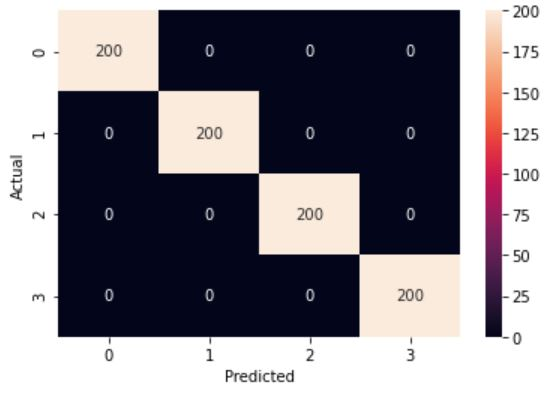
\includegraphics[scale=0.5]{dataset1a_mlffnn_cm_train.jpg}
	\caption{Training data}
	\label{fig:fig1.2.1.1}
	\end{subfigure}
	\begin{subfigure}[b]{0.45\textwidth}
	\centering
	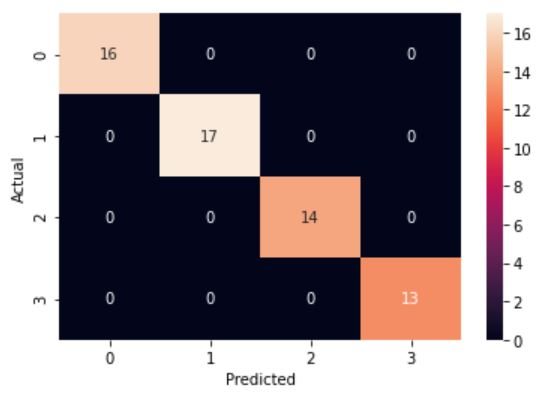
\includegraphics[scale=0.5]{dataset1a_mlffnn_cm_test.jpg}
	\caption{Test data}
	\label{fig:fig1.2.1.2}
	\end{subfigure}
\caption{Confusion matrix for the classification of dataset 1a using mlffnn with 3 nodes in hidden layer}
\label{fig:fig1.2.1}
\end{figure}

\begin{figure}[h]
\centering
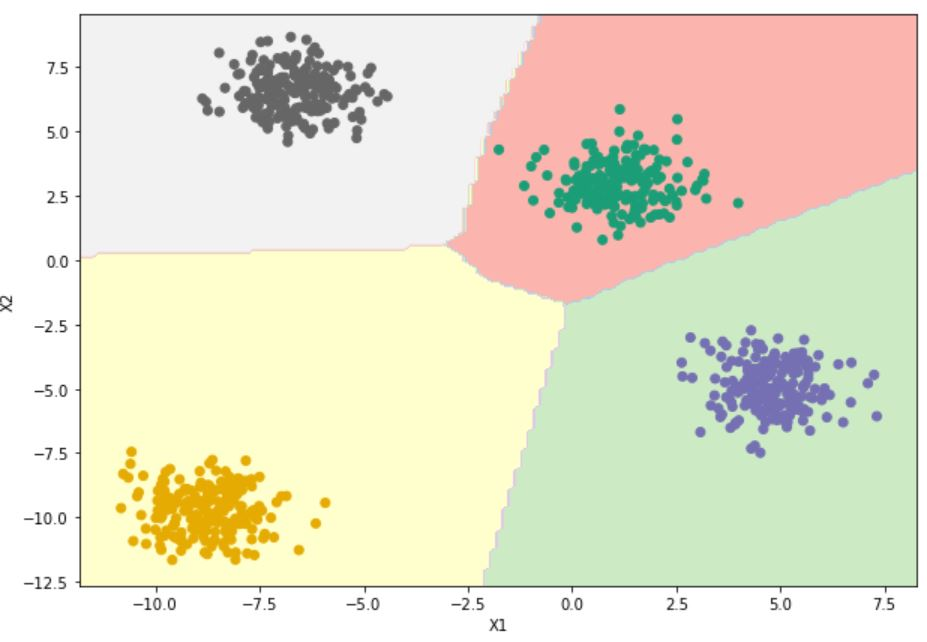
\includegraphics[scale=0.3]{dataset1a_mlffnn_ds.jpg}
\caption{Decision surfaces for plots of dataset 1a using mlffnn with 3 nodes in hidden layer}
\label{fig:fig1.2.2}
\end{figure}
\newpage

\subsection{Linear SVM classifier for every pair of class}
Hyperparameter $C = \{0.1,1\}$\\

Since the classes are linearly well separated we got the same accuracies for each value of $C$.
\begin{table}[h!]
\label{tab:tab1.3.1}
\begin{center}
\begin{tabular}{|l|c|c|c|}
\hline
\textbf{classes} & \textbf{Training Dataset} & \textbf{Validation Dataset} &\textbf{Test Dataset}\\
\hline
0 vs 1 & 100 & 100 & 100\\
\hline
0 vs 2 & 100 & 100 & 100\\
\hline
0 vs 3 & 100 & 100 & 100\\
\hline
1 vs 2 & 100 & 100 & 100\\
\hline
1 vs 3 & 100 & 100 & 100\\
\hline
2 vs 3 & 100 & 100 & 100\\
\hline
\end{tabular}
\caption{Classification accuracy using linear SVM on Dataset 1a}
\end{center}
\end{table}

As we can see from the table above the model with the best performance on the test data is with  $\eta =1$ with an accuracy of 100\% for all pairs of classes .
\begin{figure}[h]
\centering
	\begin{subfigure}[b]{0.45\textwidth}
	\centering
	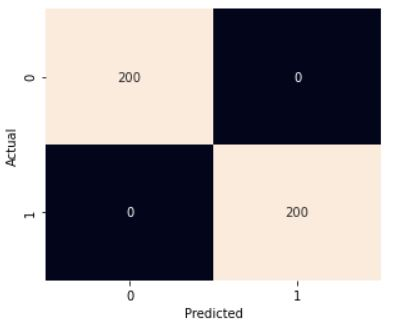
\includegraphics[scale=0.45]{dataset1a_linear_svm_01_cm_train.jpg}
	\caption{Training data}
	\label{fig:fig1.3.1.1}
	\end{subfigure}
	\begin{subfigure}[b]{0.45\textwidth}
	\centering
	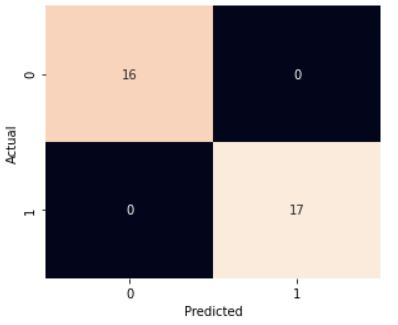
\includegraphics[scale=0.45]{dataset1a_linear_svm_01_cm_test.jpg}
	\caption{Test data}
	\label{fig:fig1.3.1.2}
	\end{subfigure}
\caption{Confusion matrix for the classification between class 0 vs class 1 of dataset 1a using linear SVM}
\label{fig:fig1.3.1}
\end{figure}

\begin{figure}[h]
\centering
	\begin{subfigure}[b]{0.45\textwidth}
	\centering
	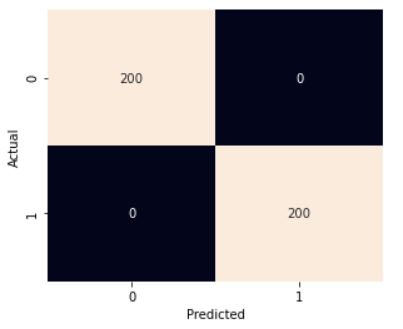
\includegraphics[scale=0.4]{dataset1a_linear_svm_02_cm_train.jpg}
	\caption{Training data}
	\label{fig:fig1.3.2.1}
	\end{subfigure}
	\begin{subfigure}[b]{0.45\textwidth}
	\centering
	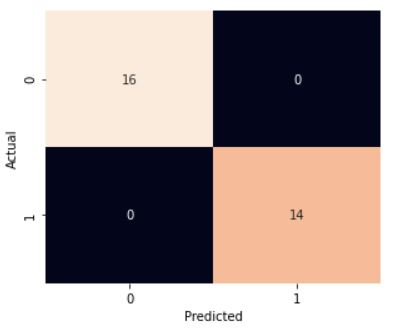
\includegraphics[scale=0.4]{dataset1a_linear_svm_02_cm_test.jpg}
	\caption{Test data}
	\label{fig:fig1.3.2.2}
	\end{subfigure}
\caption{Confusion matrix for the classification between class 0 vs class 2 of dataset 1a using linear SVM}
\label{fig:fig1.3.2}
\end{figure}

\newpage

\begin{figure}[h]
\centering
	\begin{subfigure}[b]{0.45\textwidth}
	\centering
	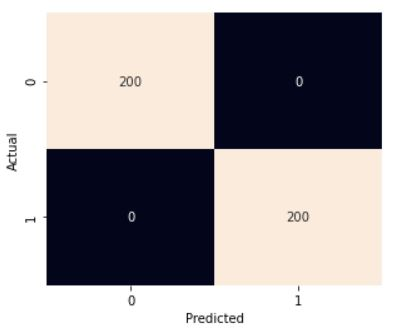
\includegraphics[scale=0.35]{dataset1a_linear_svm_03_cm_train.jpg}
	\caption{Training data}
	\label{fig:fig1.3.3.1}
	\end{subfigure}
	\begin{subfigure}[b]{0.45\textwidth}
	\centering
	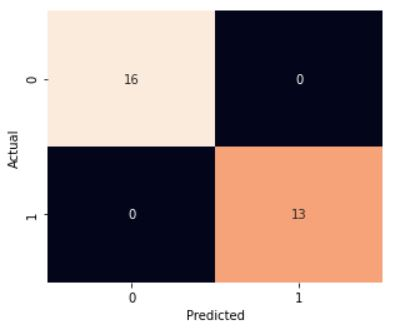
\includegraphics[scale=0.35]{dataset1a_linear_svm_03_cm_test.jpg}
	\caption{Test data}
	\label{fig:fig1.3.3.2}
	\end{subfigure}
\caption{Confusion matrix for the classification between class 0 vs class 3 of dataset 1a using linear SVM}
\label{fig:fig1.3.3}
\end{figure}

\begin{figure}[h]
\centering
	\begin{subfigure}[b]{0.45\textwidth}
	\centering
	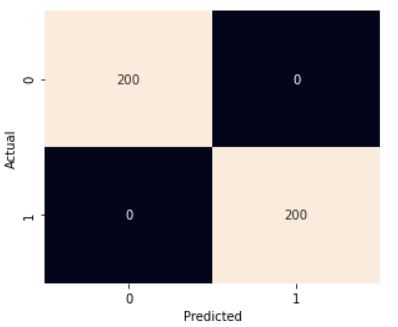
\includegraphics[scale=0.35]{dataset1a_linear_svm_12_cm_train.jpg}
	\caption{Training data}
	\label{fig:fig1.3.4.1}
	\end{subfigure}
	\begin{subfigure}[b]{0.45\textwidth}
	\centering
	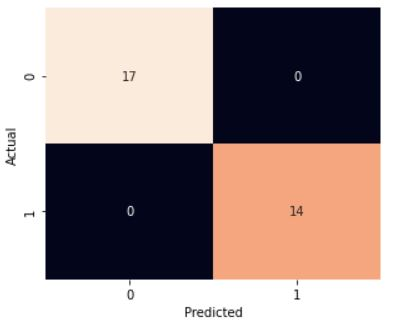
\includegraphics[scale=0.35]{dataset1a_linear_svm_12_cm_test.jpg}
	\caption{Test data}
	\label{fig:fig1.3.4.2}
	\end{subfigure}
\caption{Confusion matrix for the classification between class 1 vs class 2 of dataset 1a using linear SVM}
\label{fig:fig1.3.4}
\end{figure}

\begin{figure}[h!]
\centering
	\begin{subfigure}[b]{0.45\textwidth}
	\centering
	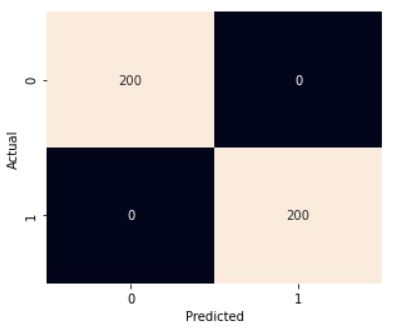
\includegraphics[scale=0.35]{dataset1a_linear_svm_13_cm_train.jpg}
	\caption{Training data}
	\label{fig:fig1.3.5.1}
	\end{subfigure}
	\begin{subfigure}[b]{0.45\textwidth}
	\centering
	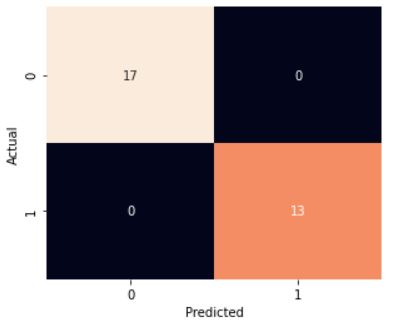
\includegraphics[scale=0.35]{dataset1a_linear_svm_13_cm_test.jpg}
	\caption{Test data}
	\label{fig:fig1.3.5.2}
	\end{subfigure}
\caption{Confusion matrix for the classification between class 1 vs class 3 of dataset 1a using linear SVM}
\label{fig:fig1.3.5}
\end{figure}

\begin{figure}[h!]
\centering
	\begin{subfigure}[b]{0.45\textwidth}
	\centering
	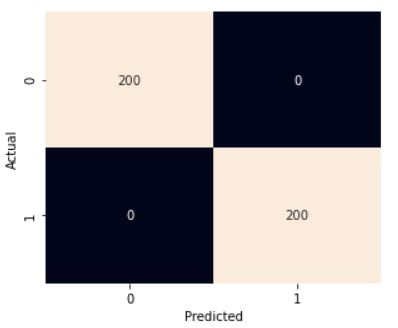
\includegraphics[scale=0.35]{dataset1a_linear_svm_23_cm_train.jpg}
	\caption{Training data}
	\label{fig:fig1.3.6.1}
	\end{subfigure}
	\begin{subfigure}[b]{0.45\textwidth}
	\centering
	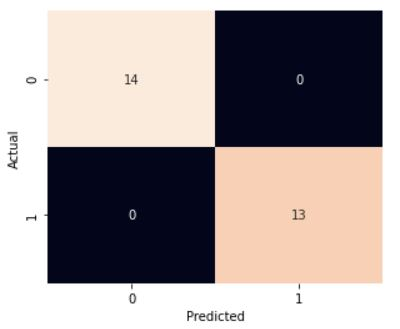
\includegraphics[scale=0.35]{dataset1a_linear_svm_23_cm_test.jpg}
	\caption{Test data}
	\label{fig:fig1.3.6.2}
	\end{subfigure}
\caption{Confusion matrix for the classification between class 2 vs class 3 of dataset 1a using linear SVM}
\label{fig:fig1.3.6}
\end{figure}

\newpage

\begin{figure}[h!]
\centering
	\begin{subfigure}[b]{0.45\textwidth}
	\centering
	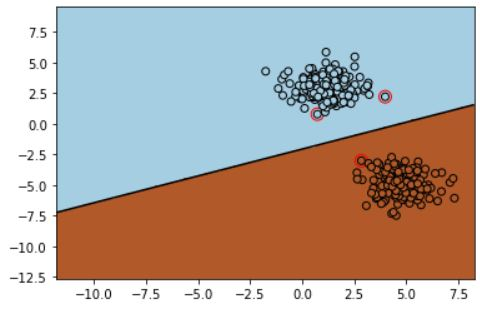
\includegraphics[scale=0.6]{dataset1a_linear_svm_01_ds.jpg}
	\caption{class 0 vs class 1}
	\label{fig:fig1.3.7.1}
	\end{subfigure}
	\begin{subfigure}[b]{0.45\textwidth}
	\centering
	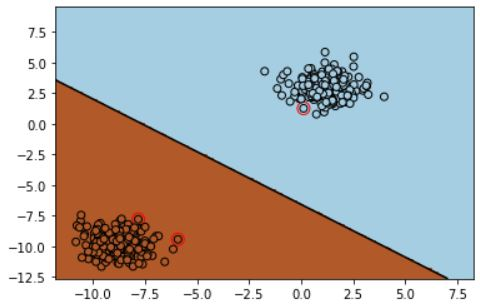
\includegraphics[scale=0.6]{dataset1a_linear_svm_02_ds.jpg}
	\caption{class 0 vs class 2}
	\label{fig:fig1.3.7.2}
	\end{subfigure}
	\begin{subfigure}[b]{0.45\textwidth}
	\centering
	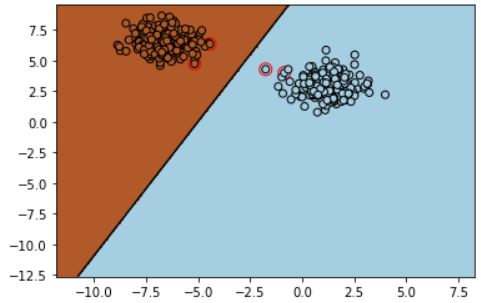
\includegraphics[scale=0.6]{dataset1a_linear_svm_03_ds.jpg}
	\caption{class 0 vs class 3}
	\label{fig:fig1.3.7.3}
	\end{subfigure}
	\begin{subfigure}[b]{0.45\textwidth}
	\centering
	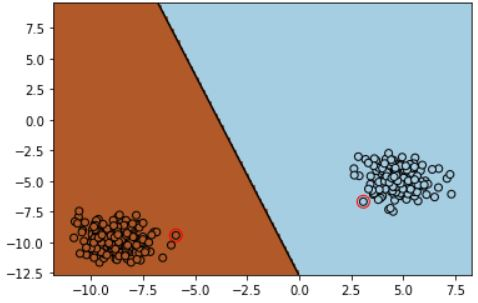
\includegraphics[scale=0.6]{dataset1a_linear_svm_12_ds.jpg}
	\caption{class 1 vs class 2}
	\label{fig:fig1.3.7.4}
	\end{subfigure}
	\begin{subfigure}[b]{0.45\textwidth}
	\centering
	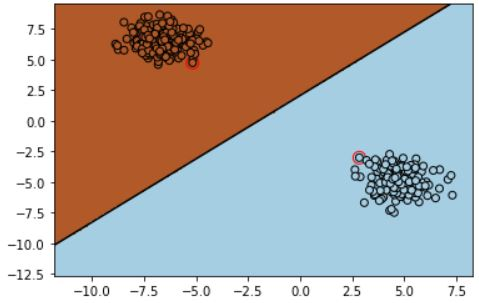
\includegraphics[scale=0.6]{dataset1a_linear_svm_13_ds.jpg}
	\caption{class 1 vs class 3}
	\label{fig:fig1.3.7.5}
	\end{subfigure}
	\begin{subfigure}[b]{0.45\textwidth}
	\centering
	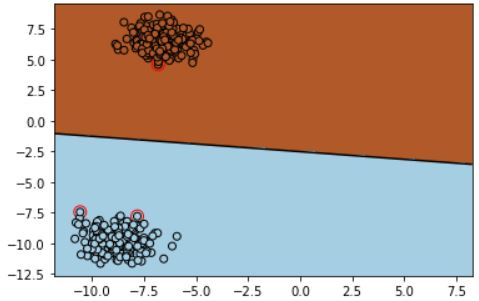
\includegraphics[scale=0.6]{dataset1a_linear_svm_23_ds.jpg}
	\caption{class 2 vs class 3}
	\label{fig:fig1.3.7.6}
	\end{subfigure}
\caption{Decision region plots between each pair of classes of dataset 1a using linear SVM}
\label{fig:fig1.3.7}
\end{figure}

Since the classes are well separated we get pretty good classification using linear SVMs and the decision surface is quite away from the data points as well.
\newpage

\section{Dataset 1b}
\subsection{MLFFNN with 2 hidden layers}

Hyperparameters : number of nodes in the hidden layers $= \{(4,2),(5,4),(6,4),(7,6)\}$\\

We used a learning rate $\eta = 0.001$, $\alpha = 1$. 
\begin{table}[h!]
\label{tab:tab2.1.1}
\begin{center}
\begin{tabular}{|l|c|c|c|c|}
\hline
\textbf{\#nodes(layer 1)} & \textbf{\#nodes(layer 2)} & \textbf{Training Dataset} & \textbf{Validation Dataset} &\textbf{Test Dataset}\\
\hline
4 & 2 &  36.56 & 33.33 & 24.44\\
\hline
5 & 4 & 93.5 & 93.33 & 88.88\\
\hline
6 & 4 & 98.83 & 97.77 & 100\\
\hline
7 & 6 & 100 & 100 & 100\\
\hline
\end{tabular}
\caption{Classification accuracy of MLFFNN with 2 hidden layer on Dataset 1b}
\end{center}
\end{table}

As we can see from the table above the model had the best classification accuracy using MLFFNN was $100\%$ when the number of nodes in the hidden layers were $7,6$ respectively.

\begin{figure}[h]
\centering
	\begin{subfigure}[b]{0.45\textwidth}
	\centering
	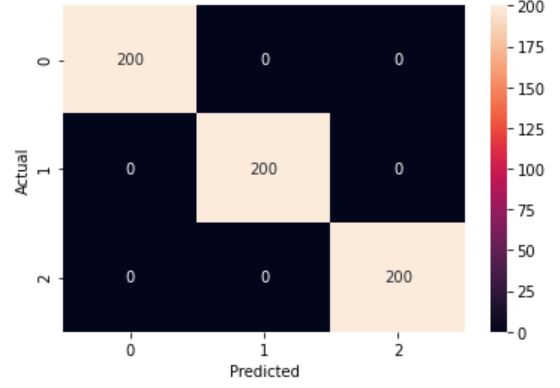
\includegraphics[scale=0.45]{dataset1b_mlffnn_cm_train.jpg}
	\caption{Training data}
	\label{fig:fig2.1.1.1}
	\end{subfigure}
	\begin{subfigure}[b]{0.45\textwidth}
	\centering
	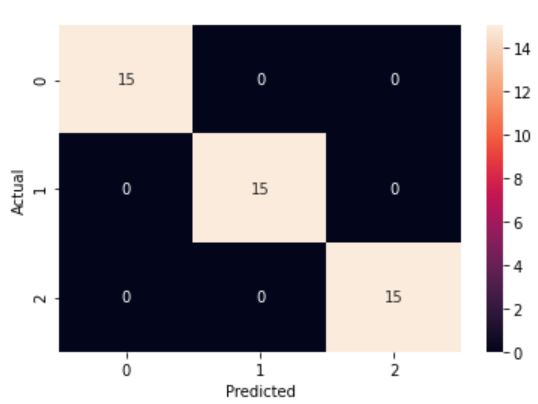
\includegraphics[scale=0.45]{dataset1b_mlffnn_cm_test.jpg}
	\caption{Test data}
	\label{fig:fig2.1.1.2}
	\end{subfigure}
\caption{Confusion matrix for datatset 1b using MLFFNN with 7 nodes in Hidden layer 1 and 6 nodes in Hidden layer 2}
\label{fig:fig2.1.1}
\end{figure}

\begin{figure}
\centering
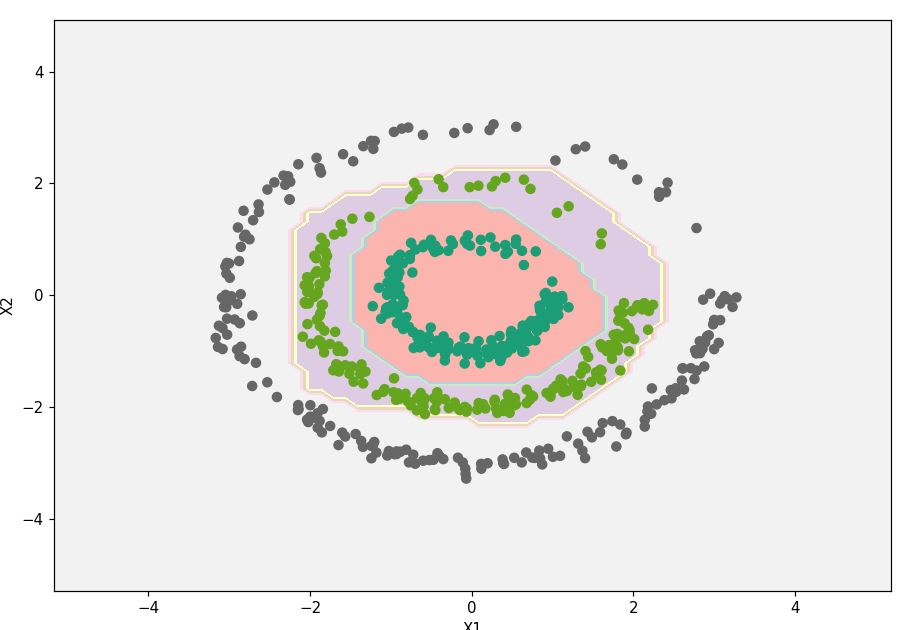
\includegraphics[scale=0.25]{dataset1b_mlffnn_ds.jpg}
\caption{Decision surfaces for plots of dataset 1b using mlffnn}
\label{fig:fig2.1.2}
\end{figure}

\newpage
\subsubsection{Output layer outputs}
 
\begin{figure}[h!]
\centering
	\begin{subfigure}[b]{0.30\textwidth}
	\centering
	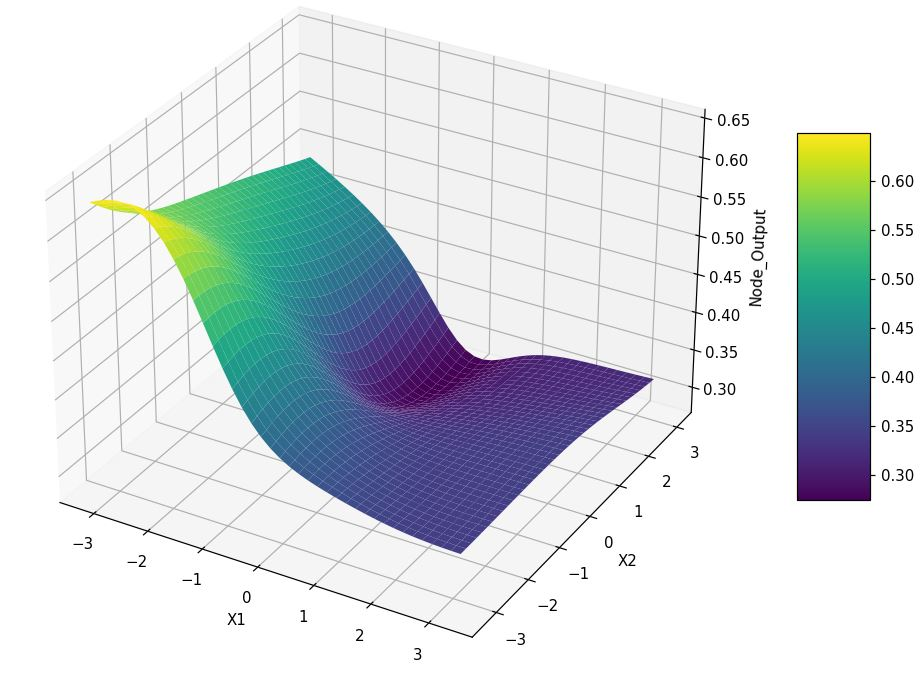
\includegraphics[scale=0.14]{output_n1_e1.jpg}
	\caption{node 1, epoch 1}
	\label{fig:fig2.1.3.1}
	\end{subfigure}
	\begin{subfigure}[b]{0.30\textwidth}
	\centering
	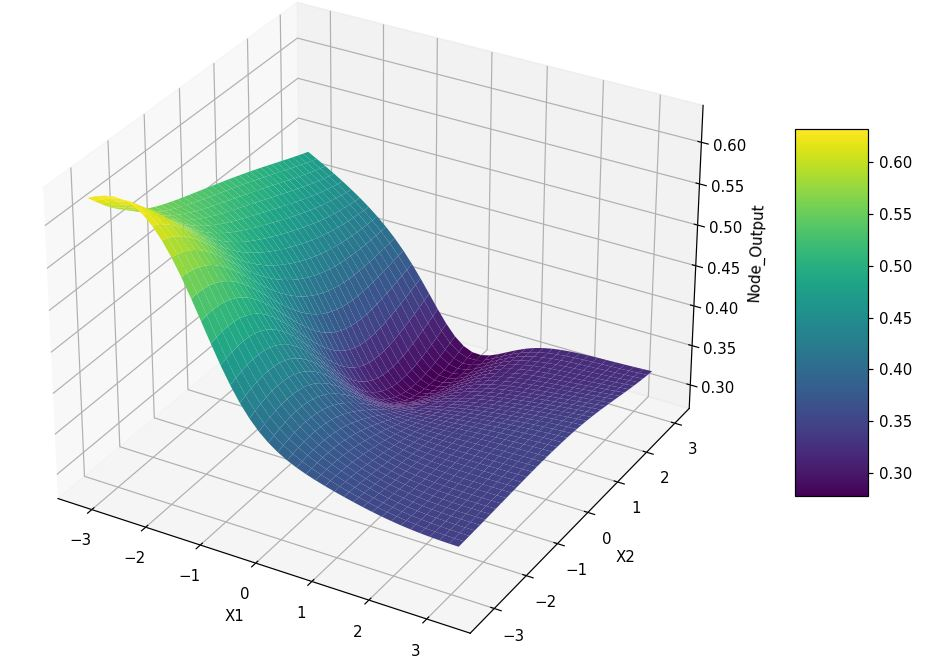
\includegraphics[scale=0.14]{output_n1_e5.jpg}
	\caption{node 1, epoch 5}
	\label{fig:fig2.1.3.2}
	\end{subfigure}
	\begin{subfigure}[b]{0.30\textwidth}
	\centering
	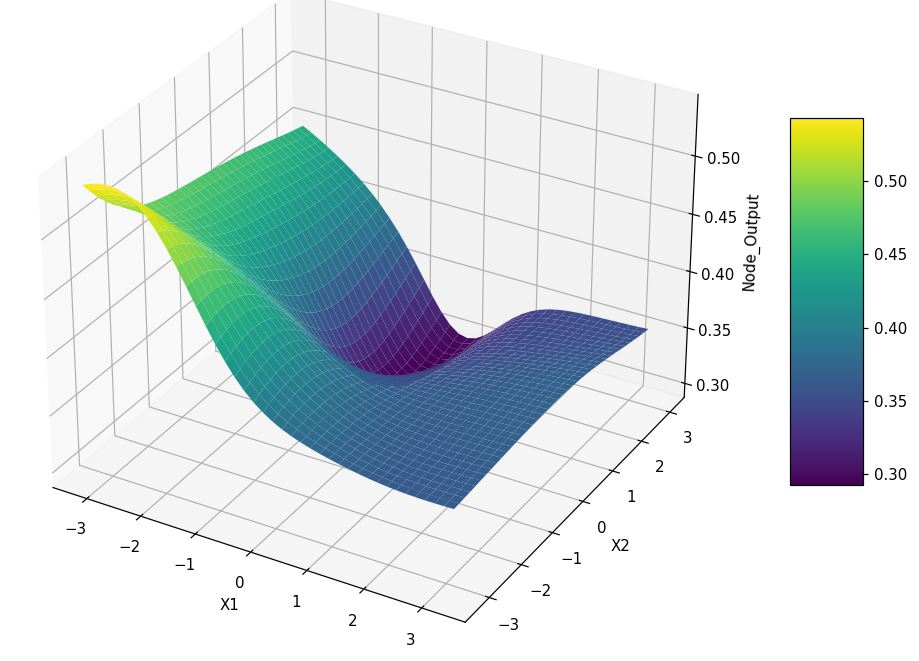
\includegraphics[scale=0.14]{output_n1_e20.jpg}
	\caption{node 1, epoch 20}
	\label{fig:fig2.1.3.3}
	\end{subfigure}
	\begin{subfigure}[b]{0.45\textwidth}
	\centering
	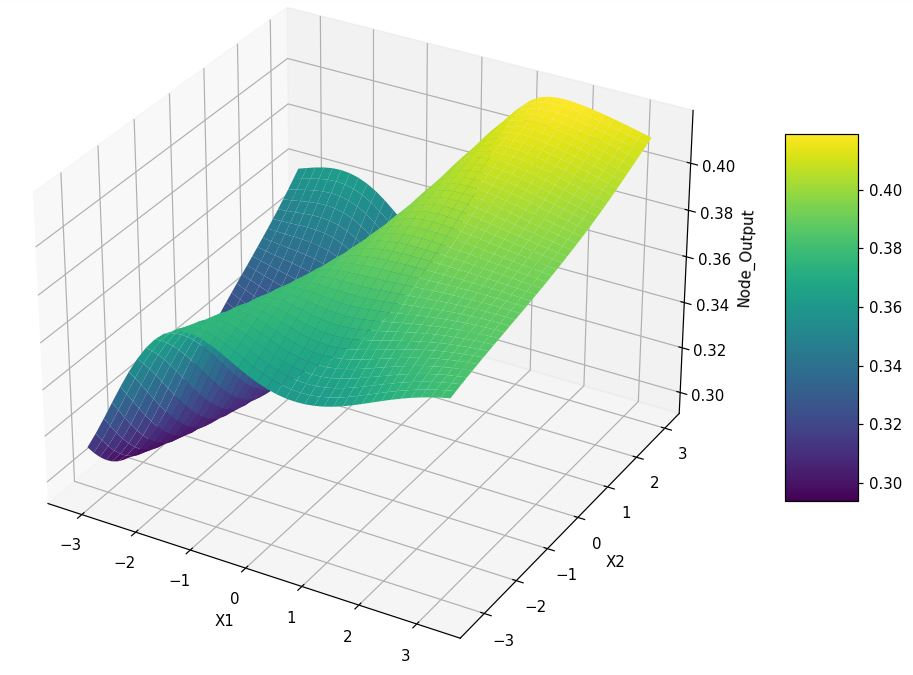
\includegraphics[scale=0.14]{output_n1_e100.jpg}
	\caption{node 1, epoch 100}
	\label{fig:fig2.1.3.4}
	\end{subfigure}
	\begin{subfigure}[b]{0.45\textwidth}
	\centering
	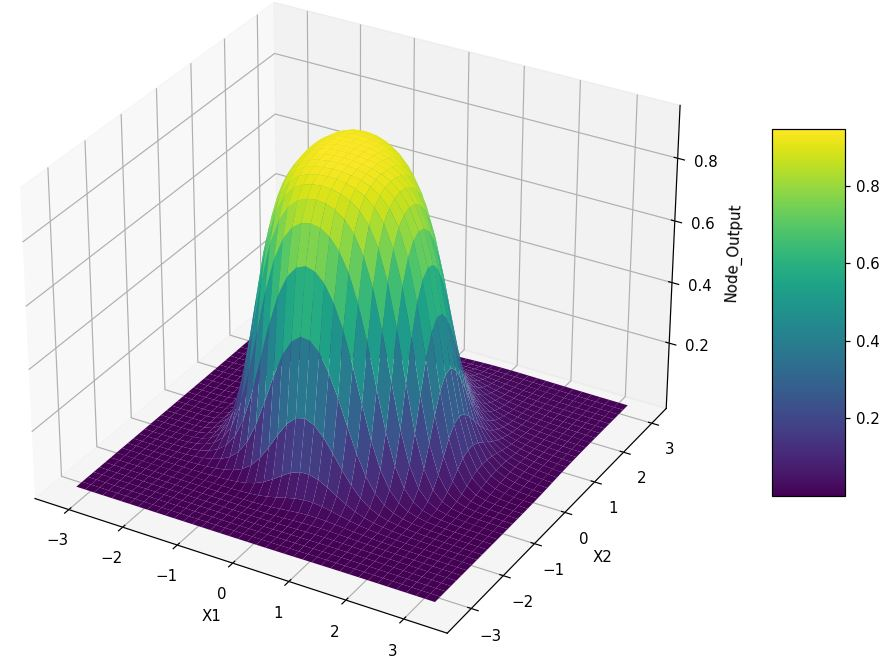
\includegraphics[scale=0.14]{output_n1_c.jpg}
	\caption{converged node 1}
	\label{fig:fig2.1.3.5}
	\end{subfigure}
	\begin{subfigure}[b]{0.30\textwidth}
	\centering
	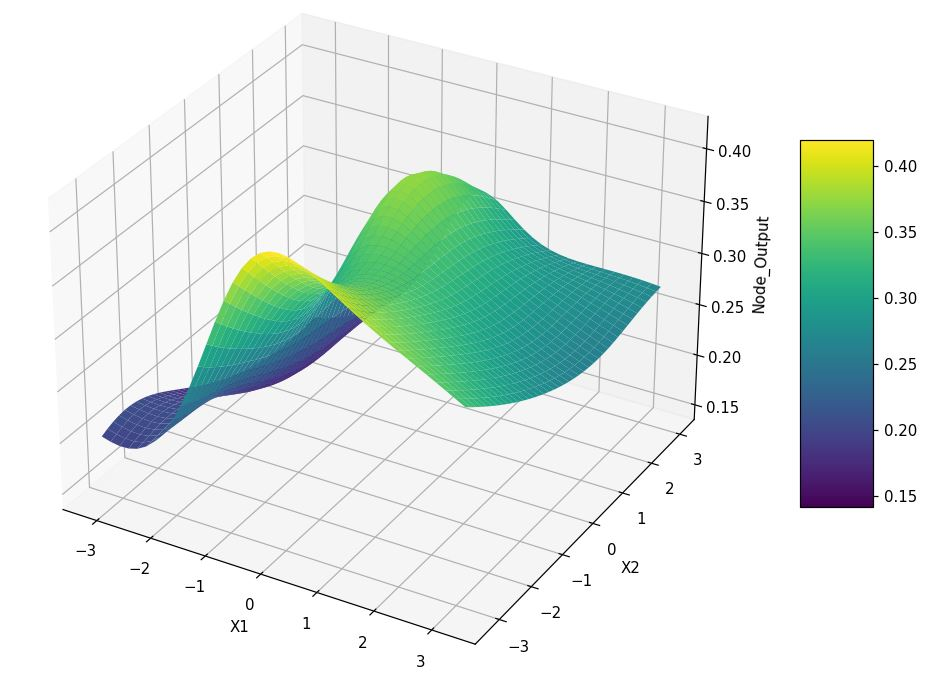
\includegraphics[scale=0.14]{output_n2_e1.jpg}
	\caption{node 2, epoch 1}
	\label{fig:fig2.1.3.6}
	\end{subfigure}
	\begin{subfigure}[b]{0.30\textwidth}
	\centering
	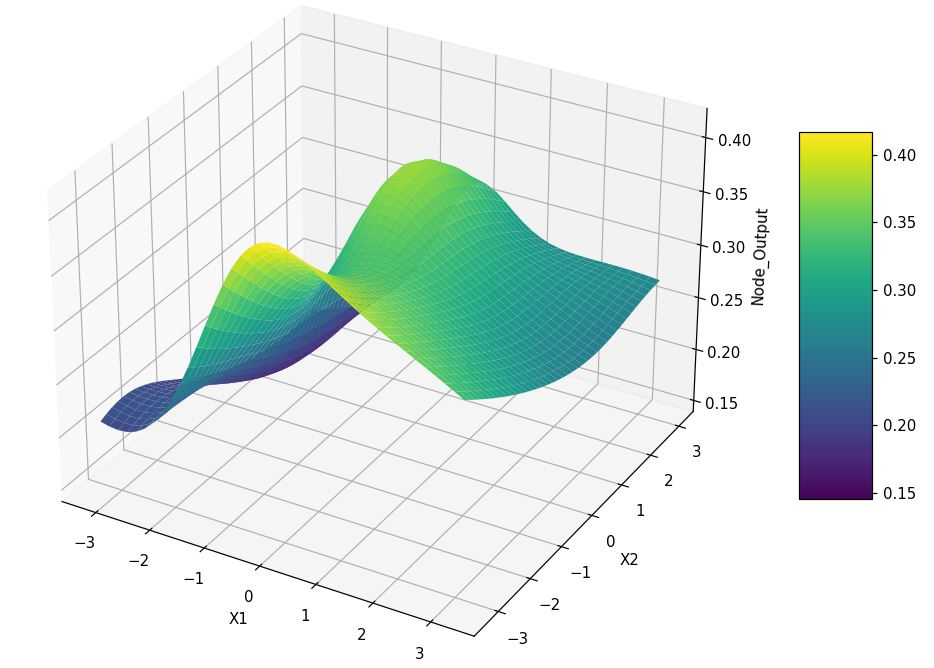
\includegraphics[scale=0.14]{output_n2_e5.jpg}
	\caption{node 2, epoch 5}
	\label{fig:fig2.1.3.7}
	\end{subfigure}
	\begin{subfigure}[b]{0.30\textwidth}
	\centering
	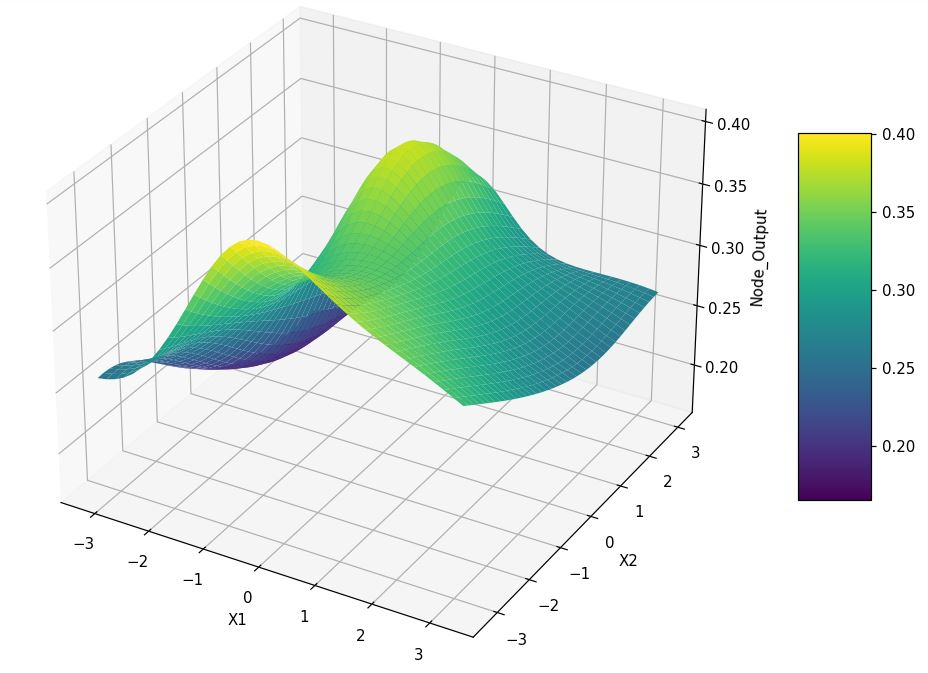
\includegraphics[scale=0.14]{output_n2_e20.jpg}
	\caption{node 2, epoch 20}
	\label{fig:fig2.1.3.8}
	\end{subfigure}
	\begin{subfigure}[b]{0.45\textwidth}
	\centering
	\includegraphics[scale=0.14]{output_n2_e100.jpg}
	\caption{node 2, epoch 100}
	\label{fig:fig2.1.3.9}
	\end{subfigure}
	\begin{subfigure}[b]{0.45\textwidth}
	\centering
	\includegraphics[scale=0.14]{output_n2_c.jpg}
	\caption{ converged node 2}
	\label{fig:fig2.1.3.10}
	\end{subfigure}
	\begin{subfigure}[b]{0.30\textwidth}
	\centering
	\includegraphics[scale=0.14]{output_n3_e1.jpg}
	\caption{node 3, epoch 1}
	\label{fig:fig2.1.3.11}
	\end{subfigure}
	\begin{subfigure}[b]{0.30\textwidth}
	\centering
	\includegraphics[scale=0.14]{output_n3_e5.jpg}
	\caption{ node 3, epoch 5}
	\label{fig:fig2.1.3.12}
	\end{subfigure}
	\begin{subfigure}[b]{0.30\textwidth}
	\centering
	\includegraphics[scale=0.14]{output_n3_e20.jpg}
	\caption{node 3, epoch 20}
	\label{fig:fig2.1.3.13}
	\end{subfigure}
	\begin{subfigure}[b]{0.45\textwidth}
	\centering
	\includegraphics[scale=0.14]{output_n3_e100.jpg}
	\caption{node 3, epoch 100}
	\label{fig:fig2.1.3.14}
	\end{subfigure}
	\begin{subfigure}[b]{0.45\textwidth}
	\centering
	\includegraphics[scale=0.14]{output_n3_c.jpg}
	\caption{converged node 3}
	\label{fig:fig2.1.3.15}
	\end{subfigure}
\caption{Outputs of the output nodes for datatset 1b using MLFFNN with 7 nodes in Hidden layer 1 and 6 nodes in Hidden layer 2}
\label{fig:fig2.1.3}
\end{figure}
We can see the output of each of the node in the output layer through different number of Epochs completed during the classification done using MLFFNN with 2 hidden layers having $7,6$ nodes respectively.
\newpage
\subsubsection{Hidden Layer 1 outputs}
\begin{figure}[h]
\centering
	\begin{subfigure}[b]{0.18\textwidth}
	\centering
	\includegraphics[scale=0.14]{hidden1_n1_e1.jpg}
	\caption{node 1,epoch 1}
	\label{fig:fig2.1.4.1}
	\end{subfigure}
	\begin{subfigure}[b]{0.18\textwidth}
	\centering
	\includegraphics[scale=0.14]{hidden1_n1_e5.jpg}
	\caption{node 1,epoch 5}
	\label{fig:fig2.1.4.2}
	\end{subfigure}
	\begin{subfigure}[b]{0.18\textwidth}
	\centering
	\includegraphics[scale=0.14]{hidden1_n1_e20.jpg}
	\caption{node 1,epoch 20}
	\label{fig:fig2.1.4.3}
	\end{subfigure}
	\begin{subfigure}[b]{0.18\textwidth}
	\centering
	\includegraphics[scale=0.14]{hidden1_n1_e100.jpg}
	\caption{node 1, epoch 100}
	\label{fig:fig2.1.4.4}
	\end{subfigure}
	\begin{subfigure}[b]{0.18\textwidth}
	\centering
	\includegraphics[scale=0.14]{hidden1_n1_c.jpg}
	\caption{converged node 1}
	\label{fig:fig2.1.4.5}
	\end{subfigure}
	\begin{subfigure}[b]{0.18\textwidth}
	\centering
	\includegraphics[scale=0.14]{hidden1_n2_e1.jpg}
	\caption{node 2, epoch 1}
	\label{fig:fig2.1.4.6}
	\end{subfigure}
	\begin{subfigure}[b]{0.18\textwidth}
	\centering
	\includegraphics[scale=0.14]{hidden1_n2_e5.jpg}
	\caption{node 2, epoch 5}
	\label{fig:fig2.1.4.7}
	\end{subfigure}
	\begin{subfigure}[b]{0.18\textwidth}
	\centering
	\includegraphics[scale=0.14]{hidden1_n2_e20.jpg}
	\caption{node 2, epoch 20}
	\label{fig:fig2.1.4.8}
	\end{subfigure}
	\begin{subfigure}[b]{0.18\textwidth}
	\centering
	\includegraphics[scale=0.14]{hidden1_n2_e100.jpg}
	\caption{node 2, epoch 100}
	\label{fig:fig2.1.4.9}
	\end{subfigure}
	\begin{subfigure}[b]{0.18\textwidth}
	\centering
	\includegraphics[scale=0.14]{hidden1_n2_c.jpg}
	\caption{converged node 2}
	\label{fig:fig2.1.4.10}
	\end{subfigure}
	\begin{subfigure}[b]{0.18\textwidth}
	\centering
	\includegraphics[scale=0.14]{hidden1_n3_e1.jpg}
	\caption{node 3, epoch 1}
	\label{fig:fig2.1.4.11}
	\end{subfigure}
	\begin{subfigure}[b]{0.18\textwidth}
	\centering
	\includegraphics[scale=0.14]{hidden1_n3_e5.jpg}
	\caption{node 3, epoch 5}
	\label{fig:fig2.1.4.12}
	\end{subfigure}
	\begin{subfigure}[b]{0.18\textwidth}
	\centering
	\includegraphics[scale=0.14]{hidden1_n3_e20.jpg}
	\caption{node 3, epoch 20}
	\label{fig:fig2.1.4.13}
	\end{subfigure}
	\begin{subfigure}[b]{0.18\textwidth}
	\centering
	\includegraphics[scale=0.14]{hidden1_n3_e100.jpg}
	\caption{node 3, epoch 100}
	\label{fig:fig2.1.4.14}
	\end{subfigure}
	\begin{subfigure}[b]{0.18\textwidth}
	\centering
	\includegraphics[scale=0.14]{hidden1_n3_c.jpg}
	\caption{converged node 3}
	\label{fig:fig2.1.4.15}
	\end{subfigure}
	\begin{subfigure}[b]{0.18\textwidth}
	\centering
	\includegraphics[scale=0.14]{hidden1_n4_e1.jpg}
	\caption{node 4, epoch 1}
	\label{fig:fig2.1.4.16}
	\end{subfigure}
	\begin{subfigure}[b]{0.18\textwidth}
	\centering
	\includegraphics[scale=0.14]{hidden1_n4_e5.jpg}
	\caption{node 4, epoch 5}
	\label{fig:fig2.1.4.17}
	\end{subfigure}
	\begin{subfigure}[b]{0.18\textwidth}
	\centering
	\includegraphics[scale=0.14]{hidden1_n4_e20.jpg}
	\caption{node 4, epoch 20}
	\label{fig:fig2.1.4.18}
	\end{subfigure}
	\begin{subfigure}[b]{0.18\textwidth}
	\centering
	\includegraphics[scale=0.14]{hidden1_n4_e100.jpg}
	\caption{node 4, epoch 100}
	\label{fig:fig2.1.4.19}
	\end{subfigure}
	\begin{subfigure}[b]{0.18\textwidth}
	\centering
	\includegraphics[scale=0.14]{hidden1_n4_c.jpg}
	\caption{converged node 4}
	\label{fig:fig2.1.4.20}
	\end{subfigure}
\caption{Outputs of the hidden layer 1 nodes (1-4) for datatset 1b using MLFFNN with 7 nodes in Hidden layer 1 and 6 nodes in Hidden layer 2}
\label{fig:fig2.1.4}
\end{figure}

\newpage
\begin{figure}[h!]
\centering
	\begin{subfigure}[b]{0.3\textwidth}
	\centering
	\includegraphics[scale=0.14]{hidden1_n5_e1.jpg}
	\caption{node 5, epoch 1}
	\label{fig:fig2.1.5.1}
	\end{subfigure}
	\begin{subfigure}[b]{0.3\textwidth}
	\centering
	\includegraphics[scale=0.14]{hidden1_n5_e5.jpg}
	\caption{node 5, epoch 5}
	\label{fig:fig2.1.5.2}
	\end{subfigure}
	\begin{subfigure}[b]{0.3\textwidth}
	\centering
	\includegraphics[scale=0.14]{hidden1_n5_e20.jpg}
	\caption{node 5, epoch 20}
	\label{fig:fig2.1.5.3}
	\end{subfigure}
	\begin{subfigure}[b]{0.45\textwidth}
	\centering
	\includegraphics[scale=0.14]{hidden1_n5_e100.jpg}
	\caption{node 5, epoch 100}
	\label{fig:fig2.1.5.4}
	\end{subfigure}
	\begin{subfigure}[b]{0.45\textwidth}
	\centering
	\includegraphics[scale=0.14]{hidden1_n5_c.jpg}
	\caption{converged node 5}
	\label{fig:fig2.1.5.5}
	\end{subfigure}
	\begin{subfigure}[b]{0.3\textwidth}
	\centering
	\includegraphics[scale=0.14]{hidden1_n6_e1.jpg}
	\caption{node 6, epoch 1}
	\label{fig:fig2.1.5.6}
	\end{subfigure}
	\begin{subfigure}[b]{0.3\textwidth}
	\centering
	\includegraphics[scale=0.14]{hidden1_n6_e5.jpg}
	\caption{node 6, epoch 5}
	\label{fig:fig2.1.5.7}
	\end{subfigure}
	\begin{subfigure}[b]{0.3\textwidth}
	\centering
	\includegraphics[scale=0.14]{hidden1_n6_e20.jpg}
	\caption{node 6, epoch 20}
	\label{fig:fig2.1.5.8}
	\end{subfigure}
	\begin{subfigure}[b]{0.45\textwidth}
	\centering
	\includegraphics[scale=0.14]{hidden1_n6_e100.jpg}
	\caption{node 6, epoch 100}
	\label{fig:fig2.1.5.9}
	\end{subfigure}
	\begin{subfigure}[b]{0.45\textwidth}
	\centering
	\includegraphics[scale=0.14]{hidden1_n6_c.jpg}
	\caption{converged node 6}
	\label{fig:fig2.1.5.10}
	\end{subfigure}
	\begin{subfigure}[b]{0.3\textwidth}
	\centering
	\includegraphics[scale=0.14]{hidden1_n7_e1.jpg}
	\caption{node 7, epoch 1}
	\label{fig:fig2.1.5.11}
	\end{subfigure}
	\begin{subfigure}[b]{0.3\textwidth}
	\centering
	\includegraphics[scale=0.14]{hidden1_n7_e5.jpg}
	\caption{node 7, epoch 5}
	\label{fig:fig2.1.5.12}
	\end{subfigure}
	\begin{subfigure}[b]{0.3\textwidth}
	\centering
	\includegraphics[scale=0.14]{hidden1_n7_e20.jpg}
	\caption{node 7, epoch 20}
	\label{fig:fig2.1.5.13}
	\end{subfigure}
	\begin{subfigure}[b]{0.45\textwidth}
	\centering
	\includegraphics[scale=0.14]{hidden1_n7_e100.jpg}
	\caption{node 7,epoch 100}
	\label{fig:fig2.1.5.14}
	\end{subfigure}
	\begin{subfigure}[b]{0.45\textwidth}
	\centering
	\includegraphics[scale=0.14]{hidden1_n7_c.jpg}
	\caption{converged node 7}
	\label{fig:fig2.1.5.15}
	\end{subfigure}
\caption{Outputs of the hidden layer 1 nodes(5-7) for datatset 1b using MLFFNN with 7 nodes in Hidden layer 1 and 6 nodes in Hidden layer 2}
\label{fig:fig2.1.5}
\end{figure}

\newpage
\subsubsection{Hidden layer 2 outputs}
\begin{figure}[h!]
\centering
	\begin{subfigure}[b]{0.3\textwidth}
	\centering
	\includegraphics[scale=0.14]{hidden2_n1_e1.jpg}
	\caption{node 1, epoch 1}
	\label{fig:fig2.1.6.1}
	\end{subfigure}
	\begin{subfigure}[b]{0.3\textwidth}
	\centering
	\includegraphics[scale=0.14]{hidden2_n1_e5.jpg}
	\caption{node 1, epoch 5}
	\label{fig:fig2.1.6.2}
	\end{subfigure}
	\begin{subfigure}[b]{0.3\textwidth}
	\centering
	\includegraphics[scale=0.14]{hidden2_n1_e20.jpg}
	\caption{node 1, epoch 20}
	\label{fig:fig2.1.6.3}
	\end{subfigure}
	\begin{subfigure}[b]{0.45\textwidth}
	\centering
	\includegraphics[scale=0.14]{hidden2_n1_e100.jpg}
	\caption{node 1, epoch 100}
	\label{fig:fig2.1.6.4}
	\end{subfigure}
	\begin{subfigure}[b]{0.45\textwidth}
	\centering
	\includegraphics[scale=0.14]{hidden2_n1_c.jpg}
	\caption{converged node 1}
	\label{fig:fig2.1.6.5}
	\end{subfigure}
	\begin{subfigure}[b]{0.3\textwidth}
	\centering
	\includegraphics[scale=0.14]{hidden2_n2_e1.jpg}
	\caption{node 2, epoch 1}
	\label{fig:fig2.1.6.6}
	\end{subfigure}
	\begin{subfigure}[b]{0.3\textwidth}
	\centering
	\includegraphics[scale=0.14]{hidden2_n2_e5.jpg}
	\caption{node 2, epoch 5}
	\label{fig:fig2.1.6.7}
	\end{subfigure}
	\begin{subfigure}[b]{0.3\textwidth}
	\centering
	\includegraphics[scale=0.14]{hidden2_n2_e20.jpg}
	\caption{node 2, epoch 20}
	\label{fig:fig2.1.6.8}
	\end{subfigure}
	\begin{subfigure}[b]{0.45\textwidth}
	\centering
	\includegraphics[scale=0.14]{hidden2_n2_e100.jpg}
	\caption{node 2, epoch 100}
	\label{fig:fig2.1.6.9}
	\end{subfigure}
	\begin{subfigure}[b]{0.45\textwidth}
	\centering
	\includegraphics[scale=0.14]{hidden2_n2_c.jpg}
	\caption{converged node 2}
	\label{fig:fig2.1.6.10}
	\end{subfigure}
	\begin{subfigure}[b]{0.3\textwidth}
	\centering
	\includegraphics[scale=0.14]{hidden2_n3_e1.jpg}
	\caption{node 3, epoch 1}
	\label{fig:fig2.1.6.11}
	\end{subfigure}
	\begin{subfigure}[b]{0.3\textwidth}
	\centering
	\includegraphics[scale=0.14]{hidden2_n3_e5.jpg}
	\caption{node 3, epoch 5}
	\label{fig:fig2.1.6.12}
	\end{subfigure}
	\begin{subfigure}[b]{0.3\textwidth}
	\centering
	\includegraphics[scale=0.14]{hidden2_n3_e20.jpg}
	\caption{node 3, epoch 20}
	\label{fig:fig2.1.6.13}
	\end{subfigure}
	\begin{subfigure}[b]{0.45\textwidth}
	\centering
	\includegraphics[scale=0.14]{hidden2_n3_e100.jpg}
	\caption{node 3,epoch 100}
	\label{fig:fig2.1.6.14}
	\end{subfigure}
	\begin{subfigure}[b]{0.45\textwidth}
	\centering
	\includegraphics[scale=0.14]{hidden2_n3_c.jpg}
	\caption{converged node 3}
	\label{fig:fig2.1.6.15}
	\end{subfigure}
\caption{Outputs of the hidden layer 2 nodes(1-3) for datatset 1b using MLFFNN with 7 nodes in Hidden layer 1 and 6 nodes in Hidden layer 2}
\label{fig:fig2.1.6}
\end{figure}
\newpage

\begin{figure}[h!]
\centering
	\begin{subfigure}[b]{0.3\textwidth}
	\centering
	\includegraphics[scale=0.14]{hidden2_n4_e1.jpg}
	\caption{node 4, epoch 1}
	\label{fig:fig2.1.7.1}
	\end{subfigure}
	\begin{subfigure}[b]{0.3\textwidth}
	\centering
	\includegraphics[scale=0.14]{hidden2_n4_e5.jpg}
	\caption{node 4, epoch 5}
	\label{fig:fig2.1.7.2}
	\end{subfigure}
	\begin{subfigure}[b]{0.3\textwidth}
	\centering
	\includegraphics[scale=0.14]{hidden2_n4_e20.jpg}
	\caption{node 4, epoch 20}
	\label{fig:fig2.1.7.3}
	\end{subfigure}
	\begin{subfigure}[b]{0.45\textwidth}
	\centering
	\includegraphics[scale=0.14]{hidden2_n4_e100.jpg}
	\caption{node 4, epoch 100}
	\label{fig:fig2.1.7.4}
	\end{subfigure}
	\begin{subfigure}[b]{0.45\textwidth}
	\centering
	\includegraphics[scale=0.14]{hidden2_n4_c.jpg}
	\caption{converged node 4}
	\label{fig:fig2.1.7.5}
	\end{subfigure}
	\begin{subfigure}[b]{0.3\textwidth}
	\centering
	\includegraphics[scale=0.14]{hidden2_n5_e1.jpg}
	\caption{node 5, epoch 1}
	\label{fig:fig2.1.7.6}
	\end{subfigure}
	\begin{subfigure}[b]{0.3\textwidth}
	\centering
	\includegraphics[scale=0.14]{hidden2_n5_e5.jpg}
	\caption{node 5, epoch 5}
	\label{fig:fig2.1.7.7}
	\end{subfigure}
	\begin{subfigure}[b]{0.3\textwidth}
	\centering
	\includegraphics[scale=0.14]{hidden2_n5_e20.jpg}
	\caption{node 5, epoch 20}
	\label{fig:fig2.1.7.8}
	\end{subfigure}
	\begin{subfigure}[b]{0.45\textwidth}
	\centering
	\includegraphics[scale=0.14]{hidden2_n5_e100.jpg}
	\caption{node 5, epoch 100}
	\label{fig:fig2.1.7.9}
	\end{subfigure}
	\begin{subfigure}[b]{0.45\textwidth}
	\centering
	\includegraphics[scale=0.14]{hidden2_n5_c.jpg}
	\caption{converged node 5}
	\label{fig:fig2.1.7.10}
	\end{subfigure}
	\begin{subfigure}[b]{0.3\textwidth}
	\centering
	\includegraphics[scale=0.14]{hidden2_n6_e1.jpg}
	\caption{node 6, epoch 1}
	\label{fig:fig2.1.7.11}
	\end{subfigure}
	\begin{subfigure}[b]{0.3\textwidth}
	\centering
	\includegraphics[scale=0.14]{hidden2_n6_e5.jpg}
	\caption{node 6, epoch 5}
	\label{fig:fig2.1.7.12}
	\end{subfigure}
	\begin{subfigure}[b]{0.3\textwidth}
	\centering
	\includegraphics[scale=0.14]{hidden2_n6_e20.jpg}
	\caption{node 6, epoch 20}
	\label{fig:fig2.1.7.13}
	\end{subfigure}
	\begin{subfigure}[b]{0.45\textwidth}
	\centering
	\includegraphics[scale=0.14]{hidden2_n6_e100.jpg}
	\caption{node 6,epoch 100}
	\label{fig:fig2.1.7.14}
	\end{subfigure}
	\begin{subfigure}[b]{0.45\textwidth}
	\centering
	\includegraphics[scale=0.14]{hidden2_n6_c.jpg}
	\caption{converged node 6}
	\label{fig:fig2.1.7.15}
	\end{subfigure}
\caption{Outputs of the hidden layer 2 nodes(4-6) for datatset 1b using MLFFNN with 7 nodes in Hidden layer 1 and 6 nodes in Hidden layer 2}
\label{fig:fig2.1.7}
\end{figure}

\newpage

\subsection{Non-linear SVM using 1 vs rest, Polynomial kernel}

We used $C = 1$ and $degree = 4$ for classification using polynomial kernel in SVM. We also used the parameter to balance the number of training datapoints from both the classes. 
\begin{table}[h!]
\label{tab:tab2.2.1}
\begin{center}
\begin{tabular}{|l|c|c|c|}
\hline
\textbf{classes} & \textbf{Training Dataset} & \textbf{Validation Dataset} &\textbf{Test Dataset}\\
\hline
class 0 vs rest & 100 & 100 & 100\\
\hline
class 1 vs rest & 66.67 & 66.67 & 66.67\\
\hline
class 2 vs rest & 100 & 100 & 100\\
\hline
\end{tabular}
\caption{Classification accuracy of polynomial SVM classifier on Dataset 1b}
\end{center}
\end{table}

As we can see from the table above the model with the best performance on the test data has an accuracy of 100\%, 66.67\%, 100\% for class 0 vs rest, class 1 vs rest and class 2 vs rest respectively. 

\begin{figure}[h]
\centering
	\begin{subfigure}[b]{0.45\textwidth}
	\centering
	\includegraphics[scale=0.5]{dataset1b_poly_svm_0_cm_train.jpg}
	\caption{Training data}
	\label{fig:fig2.2.1.1}
	\end{subfigure}
	\begin{subfigure}[b]{0.45\textwidth}
	\centering
	\includegraphics[scale=0.5]{dataset1b_poly_svm_0_cm_test.jpg}
	\caption{Test data}
	\label{fig:fig2.2.1.2}
	\end{subfigure}
\caption{Confusion matrix for class 0 vs rest in datatset 1b using polynomial SVM}
\label{fig:fig2.2.1}
\end{figure}

\begin{figure}[h]
\centering
	\begin{subfigure}[b]{0.45\textwidth}
	\centering
	\includegraphics[scale=0.5]{dataset1b_poly_svm_1_cm_train.jpg}
	\caption{Training data}
	\label{fig:fig2.2.2.1}
	\end{subfigure}
	\begin{subfigure}[b]{0.45\textwidth}
	\centering
	\includegraphics[scale=0.5]{dataset1b_poly_svm_1_cm_test.jpg}
	\caption{Test data}
	\label{fig:fig2.2.2.2}
	\end{subfigure}
\caption{Confusion matrix for class 1 vs rest in datatset 1b using polynomial SVM}
\label{fig:fig2.2.2}
\end{figure}

Our classification accuracy for class 1 vs rest is not high when we used polynomial kernel in classification using SVM for any values of the hyperparameters, because class 1 is surrounded by points that don't belong to it from both inside and outside. It is quite difficult to come up with a polynomial which is able to linearly separate class 1 from the other two classes.
  
\newpage
\begin{figure}[h]
\centering
	\begin{subfigure}[b]{0.45\textwidth}
	\centering
	\includegraphics[scale=0.5]{dataset1b_poly_svm_2_cm_train.jpg}
	\caption{Training data}
	\label{fig:fig2.2.3.1}
	\end{subfigure}
	\begin{subfigure}[b]{0.45\textwidth}
	\centering
	\includegraphics[scale=0.5]{dataset1b_poly_svm_2_cm_test.jpg}
	\caption{Test data}
	\label{fig:fig2.2.3.2}
	\end{subfigure}
\caption{Confusion matrix for class 2 vs rest in datatset 1b using polynomial SVM}
\label{fig:fig2.2.3}
\end{figure}

\begin{figure}[h!]
\centering
	\begin{subfigure}[b]{0.45\textwidth}
	\centering
	\includegraphics[scale=0.7]{dataset1b_poly_svm_0_ds.jpg}
	\caption{class 0 vs rest}
	\label{fig:fig2.2.4.1}
	\end{subfigure}
	\begin{subfigure}[b]{0.45\textwidth}
	\centering
	\includegraphics[scale=0.7]{dataset1b_poly_svm_1_ds.jpg}
	\caption{class 1 vs rest}
	\label{fig:fig2.2.4.2}
	\end{subfigure}
	\begin{subfigure}[b]{0.45\textwidth}
	\centering
	\includegraphics[scale=0.7]{dataset1b_poly_svm_2_ds.jpg}
	\caption{class 2 vs rest}
	\label{fig:fig2.2.4.3}
	\end{subfigure}
\caption{Decision region plots for 1 class vs frest in datatset 1b using polynomial SVM}
\label{fig:fig2.2.4}
\end{figure}

As explained before we can observe that in the decision region plots that class 0, class 2 are easily separated from the other classes but class 1 still has some points which are on the wrong side of the separating curve. 

\newpage

\subsection{Non-linear SVM using 1 vs rest, Gaussian kernel}
Hyperparameters : $C = \{0.1,1\}$\\
We used for classification using rbf kernel in SVM. We also used the parameter to balance the number of training datapoints from both the classes. \\
We got similar accuracy for both the values of $C$.
\begin{table}[h!]
\label{tab:tab2.3.1}
\begin{center}
\begin{tabular}{|l|c|c|c|}
\hline
\textbf{classes} & \textbf{Training Dataset} & \textbf{Validation Dataset} &\textbf{Test Dataset}\\
\hline
class 0 vs rest & 100 & 100 & 100\\
\hline
class 1 vs rest & 99.83 & 100 & 100\\
\hline
class 2 vs rest & 100 & 100 & 100\\
\hline
\end{tabular}
\caption{Classification accuracy of Gaussian SVM classifier on Dataset 1b}
\end{center}
\end{table}

As we can see from the table above the model with the best performance on the test data for $C=1$ with an accuracy of 100\% for all the classes. 

\begin{figure}[h]
\centering
	\begin{subfigure}[b]{0.45\textwidth}
	\centering
	\includegraphics[scale=0.5]{dataset1b_gauss_svm_0_cm_train.jpg}
	\caption{Training data}
	\label{fig:fig2.3.1.1}
	\end{subfigure}
	\begin{subfigure}[b]{0.45\textwidth}
	\centering
	\includegraphics[scale=0.5]{dataset1b_gauss_svm_0_cm_test.jpg}
	\caption{Test data}
	\label{fig:fig2.3.1.2}
	\end{subfigure}
\caption{Confusion matrix for class 0 vs rest in datatset 1b using Gaussian SVM}
\label{fig:fig2.3.1}
\end{figure}

\begin{figure}[h!]
\centering
	\begin{subfigure}[b]{0.45\textwidth}
	\centering
	\includegraphics[scale=0.5]{dataset1b_gauss_svm_1_cm_train.jpg}
	\caption{Training data}
	\label{fig:fig2.3.2.1}
	\end{subfigure}
	\begin{subfigure}[b]{0.45\textwidth}
	\centering
	\includegraphics[scale=0.5]{dataset1b_gauss_svm_1_cm_test.jpg}
	\caption{Test data}
	\label{fig:fig2.3.2.2}
	\end{subfigure}
\caption{Confusion matrix for class 1 vs rest in datatset 1b using Gaussian SVM}
\label{fig:fig2.3.2}
\end{figure}

Unlike the polynomial kernel, Gaussian kernel is able to separate class 1 from the other 2 classes with pretty good accuracy.

\newpage
\begin{figure}
\centering
	\begin{subfigure}[b]{0.45\textwidth}
	\centering
	\includegraphics[scale=0.5]{dataset1b_gauss_svm_2_cm_train.jpg}
	\caption{Training data}
	\label{fig:fig2.3.3.1}
	\end{subfigure}
	\begin{subfigure}[b]{0.45\textwidth}
	\centering
	\includegraphics[scale=0.5]{dataset1b_gauss_svm_2_cm_test.jpg}
	\caption{Test data}
	\label{fig:fig2.3.3.2}
	\end{subfigure}
\caption{Confusion matrix for class 2 vs rest in datatset 1b using Gaussian SVM}
\label{fig:fig2.3.3}
\end{figure}
\begin{figure}[h]
\centering
	\begin{subfigure}[b]{0.45\textwidth}
	\centering
	\includegraphics[scale=0.7]{dataset1b_gauss_svm_0_ds.jpg}
	\caption{class 0 vs rest}
	\label{fig:fig2.3.4.1}
	\end{subfigure}
	\begin{subfigure}[b]{0.45\textwidth}
	\centering
	\includegraphics[scale=0.7]{dataset1b_gauss_svm_1_ds.jpg}
	\caption{class 1 vs rest}
	\label{fig:fig2.3.4.2}
	\end{subfigure}
	\begin{subfigure}[b]{0.45\textwidth}
	\centering
	\includegraphics[scale=0.7]{dataset1b_gauss_svm_2_ds.jpg}
	\caption{class 2 vs rest}
	\label{fig:fig2.3.4.3}
	\end{subfigure}
\caption{Decision region plots for 1 class vs frest in datatset 1b using Gaussian SVM}
\label{fig:fig2.3.4}
\end{figure}

\newpage

\section{Dataset 2}

The classes we had to distinguish between were:
\begin{enumerate}
\item Forest
\item Highway
\item Inside city
\item Mountain
\item Street
\end{enumerate}

\subsection{MLFFNN with 2 hidden layers}

Hyperparameters : \#nodes in hidden layers 1,2 $= \{(39,20), (40,40), (20,10), (30,30), (50,40),(70,60)\}$\\

 We used a learning rate $\eta = 0.001$, $\alpha = 1$. 
\begin{table}[h!]
\label{tab:tab3.1.1}
\begin{center}
\begin{tabular}{|l|c|c|c|c|}
\hline
\textbf{\#nodes(layer 1)} & \textbf{\#nodes(layer 2)} & \textbf{Training} & \textbf{Validation} &\textbf{Test}\\
\hline
39 & 20 &  94.5 & 58.59 & 58.97\\
\hline
40 & 40 & 94.04 & 64.33 & 62.82\\
\hline
20 & 10 & 86.35 & 59.87 & 62.17\\
\hline
30 & 30 & 91.12 & 66.24 & 62.17\\
\hline
50 & 40 & 92.5 & 63.7 & 61.9\\ 
\hline
70 & 60 & 95.14 & 63.7 & 64.74\\ 
\hline
\end{tabular}
\caption{Classification accuracy of MLFFNN with 2 hidden layers on Dataset 2}
\end{center}
\end{table}

The best classification accuracy of $64.74\%$ was observed when we used $70,60$ nodes in the hidden layers 1,2 respectively.

\begin{figure}[h]
\centering
	\begin{subfigure}[b]{0.45\textwidth}
	\centering
	\includegraphics[scale=0.55]{dataset2_mlffnn_cm_train.jpg}
	\caption{Training data}
	\label{fig:fig3.1.1.1}
	\end{subfigure}
	\begin{subfigure}[b]{0.45\textwidth}
	\centering
	\includegraphics[scale=0.55]{dataset2_mlffnn_cm_test.jpg}
	\caption{Test data}
	\label{fig:fig3.1.1.2}
	\end{subfigure}
\caption{Confusion matrix for datatset 2 using MLFFNN with 70 nodes in Hidden layer 1 and 60 nodes in Hidden layer 2}
\label{fig:fig3.1.1}
\end{figure}

\newpage
\subsection{Gaussian kernel based SVM using 1 vs rest}
We used $C =1$ for classification using rbf kernel in SVM. We also used the parameter to balance the number of training datapoints from both the classes. 
\begin{table}[h!]
\label{tab:tab3.2.1}
\begin{center}
\begin{tabular}{|l|c|c|c|}
\hline
\textbf{classes} & \textbf{Training Dataset} & \textbf{Validation Dataset} &\textbf{Test Dataset}\\
\hline
class 0 vs rest & 96.5169 & 93.6305 & 91.0256\\
\hline
class 1 vs rest & 99.5417 & 90.4458 & 87.8205\\
\hline
class 2 vs rest & 91.2007 & 80.8917 & 84.6153\\
\hline
class 3 vs rest & 94.8670 & 82.8025 & 80.1282\\
\hline
class 4 vs rest & 95.6003 & 82.8025 & 77.5641\\ 
\hline
\end{tabular}
\caption{Classification accuracy of Gaussian SVM classifier on Dataset 2}
\end{center}
\end{table}

As we can see from the table above the model with the best performance on the test data with an accuracy of $91.02\%, 87.82\%, 84.61\%, 80.12\%, 77.56\%$ for the classes 0,1,2,3,4 respectively. 

\begin{figure}[h]
\centering
	\begin{subfigure}[b]{0.45\textwidth}
	\centering
	\includegraphics[scale=0.5]{dataset2_gauss_0_cm_train.jpg}
	\caption{Training data}
	\label{fig:fig3.2.1.1}
	\end{subfigure}
	\begin{subfigure}[b]{0.45\textwidth}
	\centering
	\includegraphics[scale=0.5]{dataset2_gauss_0_cm_test.jpg}
	\caption{Test data}
	\label{fig:fig3.2.1.2}
	\end{subfigure}
\caption{Confusion matrix for class 0 vs rest in datatset 2 using Gaussian SVM}
\label{fig:fig3.2.1}
\end{figure}

\begin{figure}[h]
\centering
	\begin{subfigure}[b]{0.45\textwidth}
	\centering
	\includegraphics[scale=0.5]{dataset2_gauss_1_cm_train.jpg}
	\caption{Training data}
	\label{fig:fig3.2.2.1}
	\end{subfigure}
	\begin{subfigure}[b]{0.45\textwidth}
	\centering
	\includegraphics[scale=0.5]{dataset2_gauss_1_cm_test.jpg}
	\caption{Test data}
	\label{fig:fig3.2.2.2}
	\end{subfigure}
\caption{Confusion matrix for class 1 vs rest in datatset 2 using Gaussian SVM}
\label{fig:fig3.2.2}
\end{figure}

\begin{figure}[h]
\centering
	\begin{subfigure}[b]{0.45\textwidth}
	\centering
	\includegraphics[scale=0.5]{dataset2_gauss_2_cm_train.jpg}
	\caption{Training data}
	\label{fig:fig3.2.3.1}
	\end{subfigure}
	\begin{subfigure}[b]{0.45\textwidth}
	\centering
	\includegraphics[scale=0.5]{dataset2_gauss_2_cm_test.jpg}
	\caption{Test data}
	\label{fig:fig3.2.3.2}
	\end{subfigure}
\caption{Confusion matrix for class 2 vs rest in datatset 2 using Gaussian SVM}
\label{fig:fig3.2.3}
\end{figure}

\begin{figure}[h]
\centering
	\begin{subfigure}[b]{0.45\textwidth}
	\centering
	\includegraphics[scale=0.5]{dataset2_gauss_3_cm_train.jpg}
	\caption{Training data}
	\label{fig:fig3.2.4.1}
	\end{subfigure}
	\begin{subfigure}[b]{0.45\textwidth}
	\centering
	\includegraphics[scale=0.5]{dataset2_gauss_3_cm_test.jpg}
	\caption{Test data}
	\label{fig:fig3.2.4.2}
	\end{subfigure}
\caption{Confusion matrix for class 3 vs rest in datatset 2 using Gaussian SVM}
\label{fig:fig3.2.4}
\end{figure}

\begin{figure}[h]
\centering
	\begin{subfigure}[b]{0.45\textwidth}
	\centering
	\includegraphics[scale=0.5]{dataset2_gauss_4_cm_train.jpg}
	\caption{Training data}
	\label{fig:fig3.2.5.1}
	\end{subfigure}
	\begin{subfigure}[b]{0.45\textwidth}
	\centering
	\includegraphics[scale=0.5]{dataset2_gauss_4_cm_test.jpg}
	\caption{Test data}
	\label{fig:fig3.2.5.2}
	\end{subfigure}
\caption{Confusion matrix for class 4 vs rest in datatset 2 using Gaussian SVM}
\label{fig:fig3.2.5}
\end{figure}

\end{document}
